\begin{mdframed}
\textbf{La extensión máxima para esta sección es de 4 páginas.} Si utiliza menos páginas y explica bien sus resultados, es preferible.
\end{mdframed}

En esta sección se presentan los resultados experimentales obtenidos al ejecutar las cuatro implementaciones sobre las familias de casos generadas automáticamente. Los casos pequeños (\texttt{small}) se utilizaron para validar correctitud y comparar fuerza bruta con programación dinámica; las familias \texttt{\detokenize{vary_n}}, \texttt{\detokenize{vary_q}}, \texttt{\detokenize{vary_m}} y \texttt{\detokenize{vary_e}} se construyeron para aislar, respectivamente, la cantidad de animes, la cantidad total de capítulos, los minutos disponibles y la energía disponible.

\subsection{Síntesis global}

La Tabla~\ref{tab:resumen_global} resume el comportamiento promedio observado en las ejecuciones realizadas. La programación dinámica es claramente más costosa en tiempo y memoria que los métodos greedy, pero es la única implementación exacta; por ello se usa como referencia para evaluar la calidad de las heurísticas.

\begin{table}[ht]
\centering
\small
\begin{tabular}{lrr}
\hline
Algoritmo & Tiempo promedio (ms) & Memoria promedio (KB) \
\hline
Fuerza bruta & --- & --- \
Programación dinámica & --- & --- \
Greedy 1 & --- & --- \
Greedy 2 & --- & --- \
\hline
\end{tabular}
\caption{Resumen global de tiempo y memoria. Los valores deben leerse como promedios sobre los casos efectivamente ejecutados por cada algoritmo.}
\label{tab:resumen_global}
\end{table}

\subsection{Tiempo de ejecución}

La Figura~\ref{fig:tiempo_n} muestra el tiempo promedio según la cantidad de animes. Se observa que la programación dinámica crece de manera mucho más pronunciada que los métodos greedy, mientras que estos últimos se mantienen cercanos a una línea casi plana. Esto concuerda con la diferencia esperada entre un algoritmo exacto que explora un espacio de estados más grande y heurísticas que toman decisiones locales.

\begin{figure}[ht]
\centering
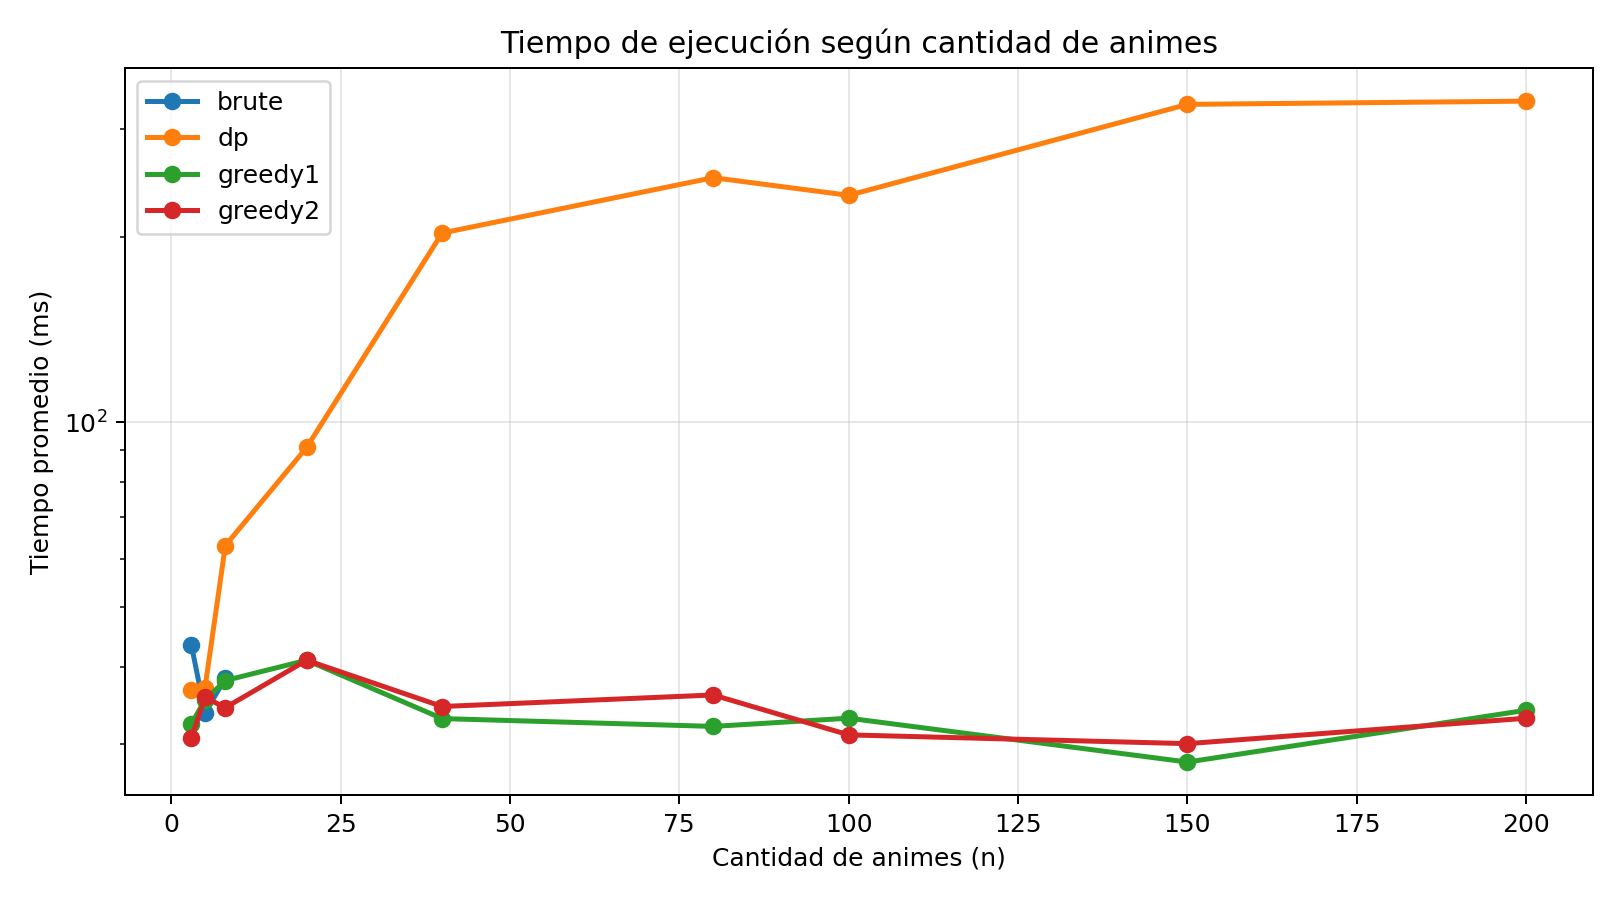
\includegraphics[width=0.92\linewidth]{../code/implementation/data/plots/tiempo_vs_n.png}
\caption{Tiempo de ejecución según cantidad de animes. La escala vertical está en logaritmo para distinguir mejor la separación entre los métodos.}
\label{fig:tiempo_n}
\end{figure}

La Figura~\ref{fig:tiempo_capitulos} presenta el tiempo según la cantidad total de capítulos. Aquí la dispersión es mayor porque esta variable no se aisló por completo: cada caso pertenece a una familia distinta y, además de variar el número de capítulos, también pueden cambiar el número de animes, los presupuestos disponibles y la distribución interna de las duraciones y energías. Aun así, se mantiene la tendencia general: programación dinámica es el método más costoso, mientras que los greedy y la fuerza bruta en casos pequeños son mucho más livianos.

\begin{figure}[ht]
\centering
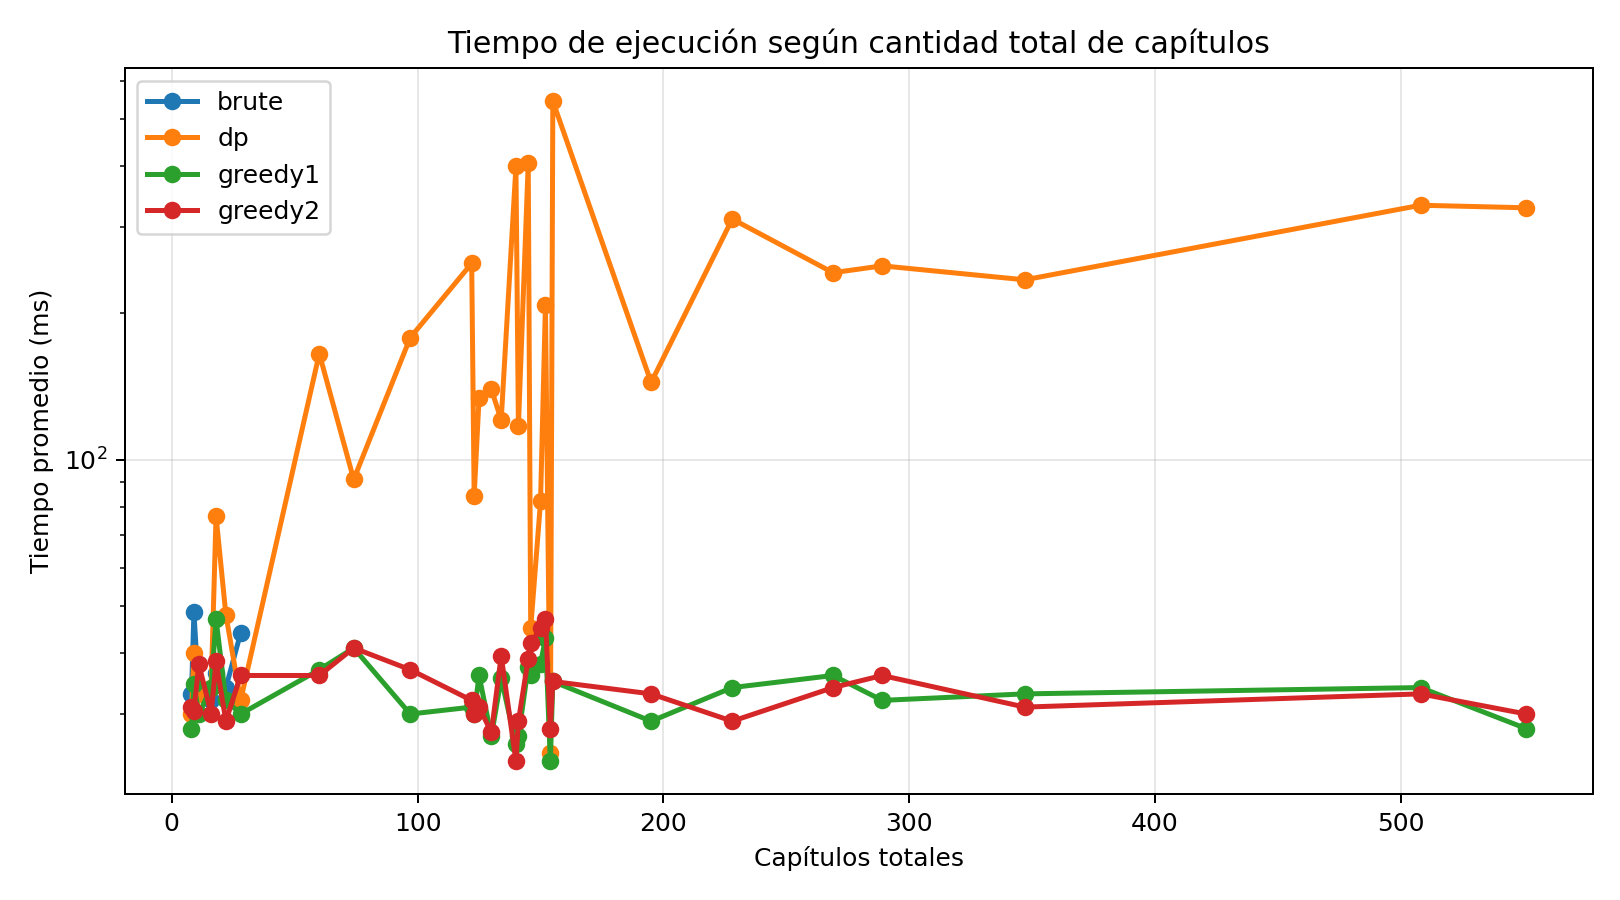
\includegraphics[width=0.92\linewidth]{../code/implementation/data/plots/tiempo_vs_capitulos.png}
\caption{Tiempo de ejecución según cantidad total de capítulos.}
\label{fig:tiempo_capitulos}
\end{figure}

Las Figuras~\ref{fig:tiempo_m} y~\ref{fig:tiempo_e} muestran el comportamiento respecto de los presupuestos de minutos y energía, respectivamente. En ambos casos la programación dinámica sigue siendo la que más se resiente cuando el espacio de estados crece, mientras que los greedy apenas cambian. Las pequeñas oscilaciones en las curvas no son una anomalía: provienen de que cada punto corresponde a una instancia distinta y, por tanto, el costo real depende también de la estructura interna de los animes y no solo del valor del presupuesto.

\begin{figure}[ht]
\centering
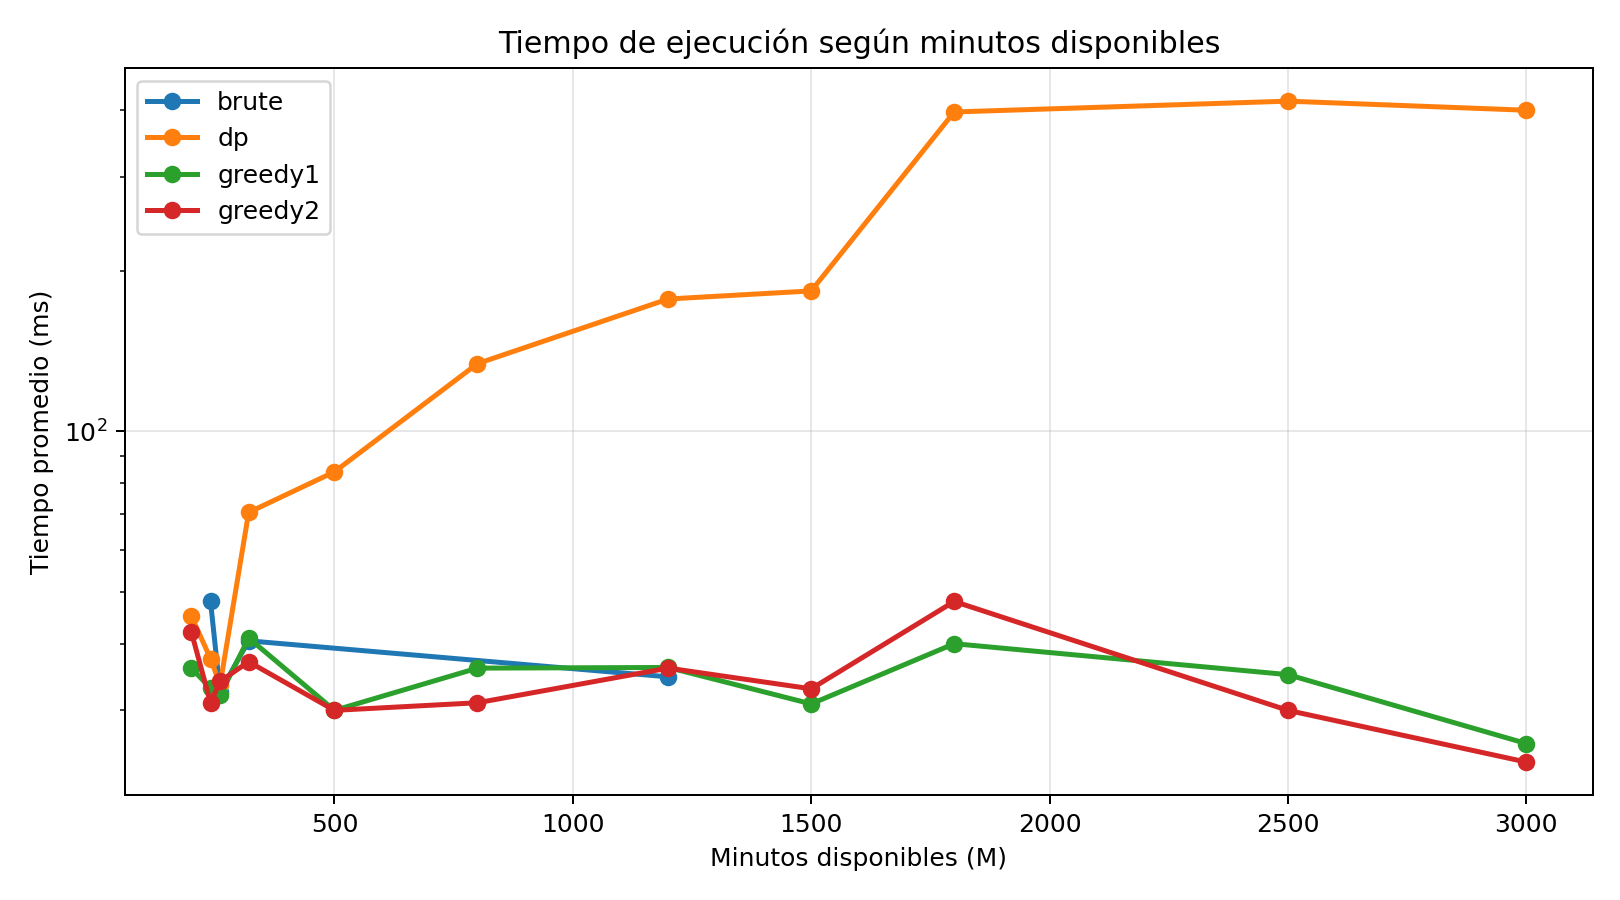
\includegraphics[width=0.92\linewidth]{../code/implementation/data/plots/tiempo_vs_M.png}
\caption{Tiempo de ejecución según minutos disponibles.}
\label{fig:tiempo_m}
\end{figure}

\begin{figure}[ht]
\centering
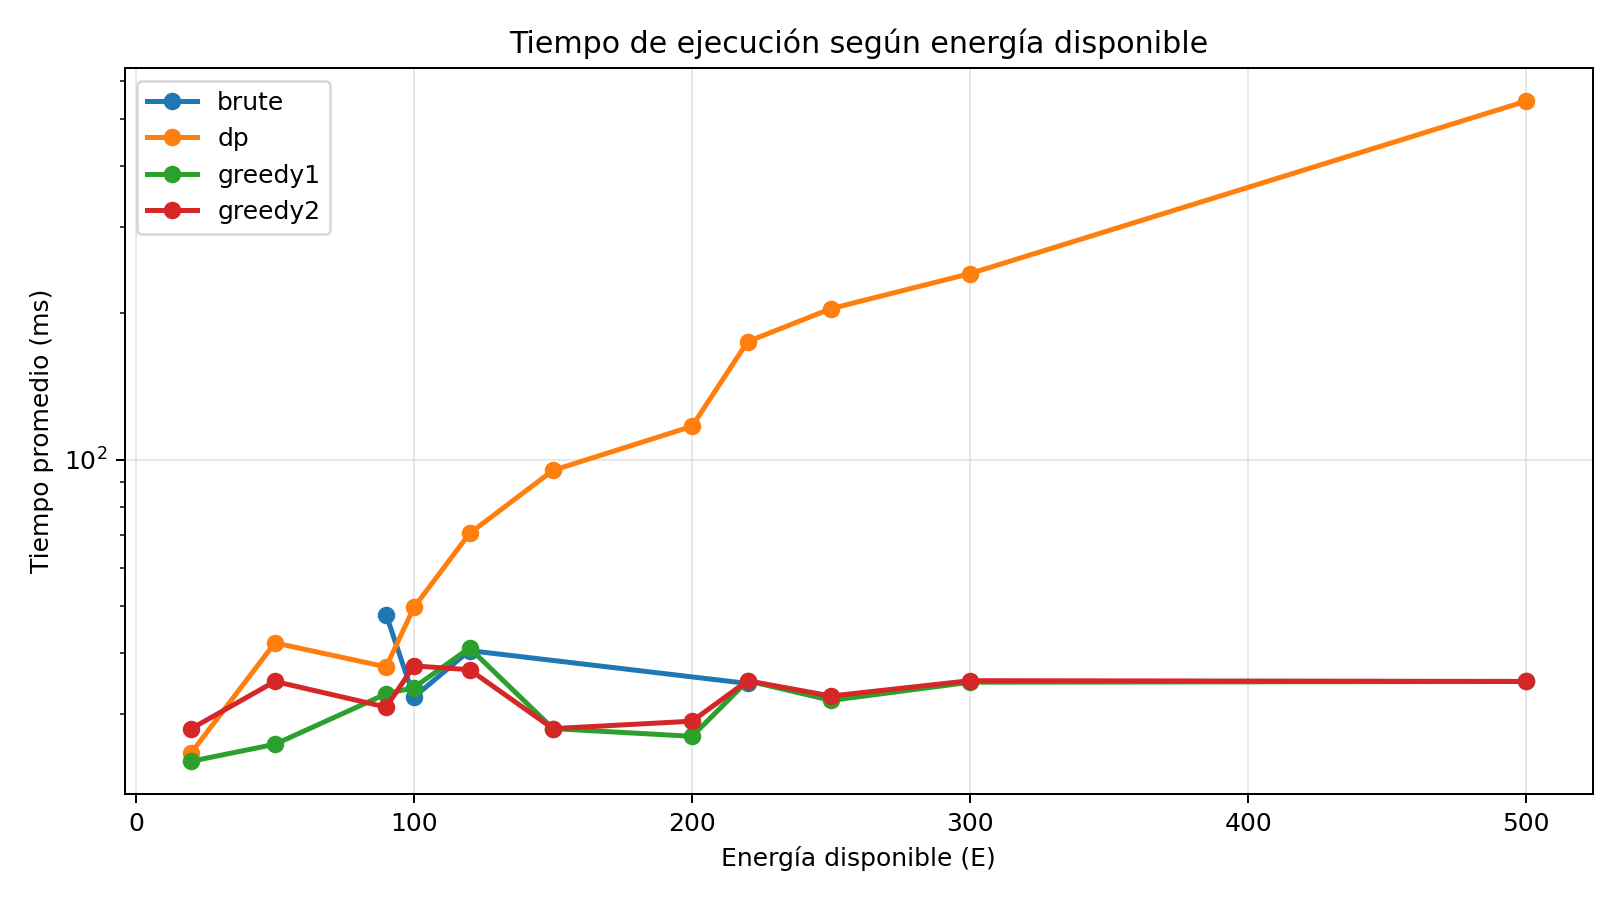
\includegraphics[width=0.92\linewidth]{../code/implementation/data/plots/tiempo_vs_E.png}
\caption{Tiempo de ejecución según energía disponible.}
\label{fig:tiempo_e}
\end{figure}

\subsection{Uso de memoria}

La memoria presenta un patrón más estable que el tiempo, aunque también exhibe variaciones entre familias. En los gráficos, los métodos greedy se mantienen cerca de un valor base muy similar entre sí, lo que es esperable porque su lógica solo requiere estructuras pequeñas para ordenar y evaluar opciones. En contraste, programación dinámica utiliza tablas de estados y, por ello, su consumo de memoria es mayor.

La Figura~\ref{fig:memoria_n} resume el uso de memoria según la cantidad de animes. Se aprecia que los greedy prácticamente permanecen en un nivel de referencia, mientras que programación dinámica incrementa su consumo a medida que crece el problema. Esto es coherente con el hecho de que DP necesita almacenar información adicional para combinar subproblemas.

\begin{figure}[ht]
\centering
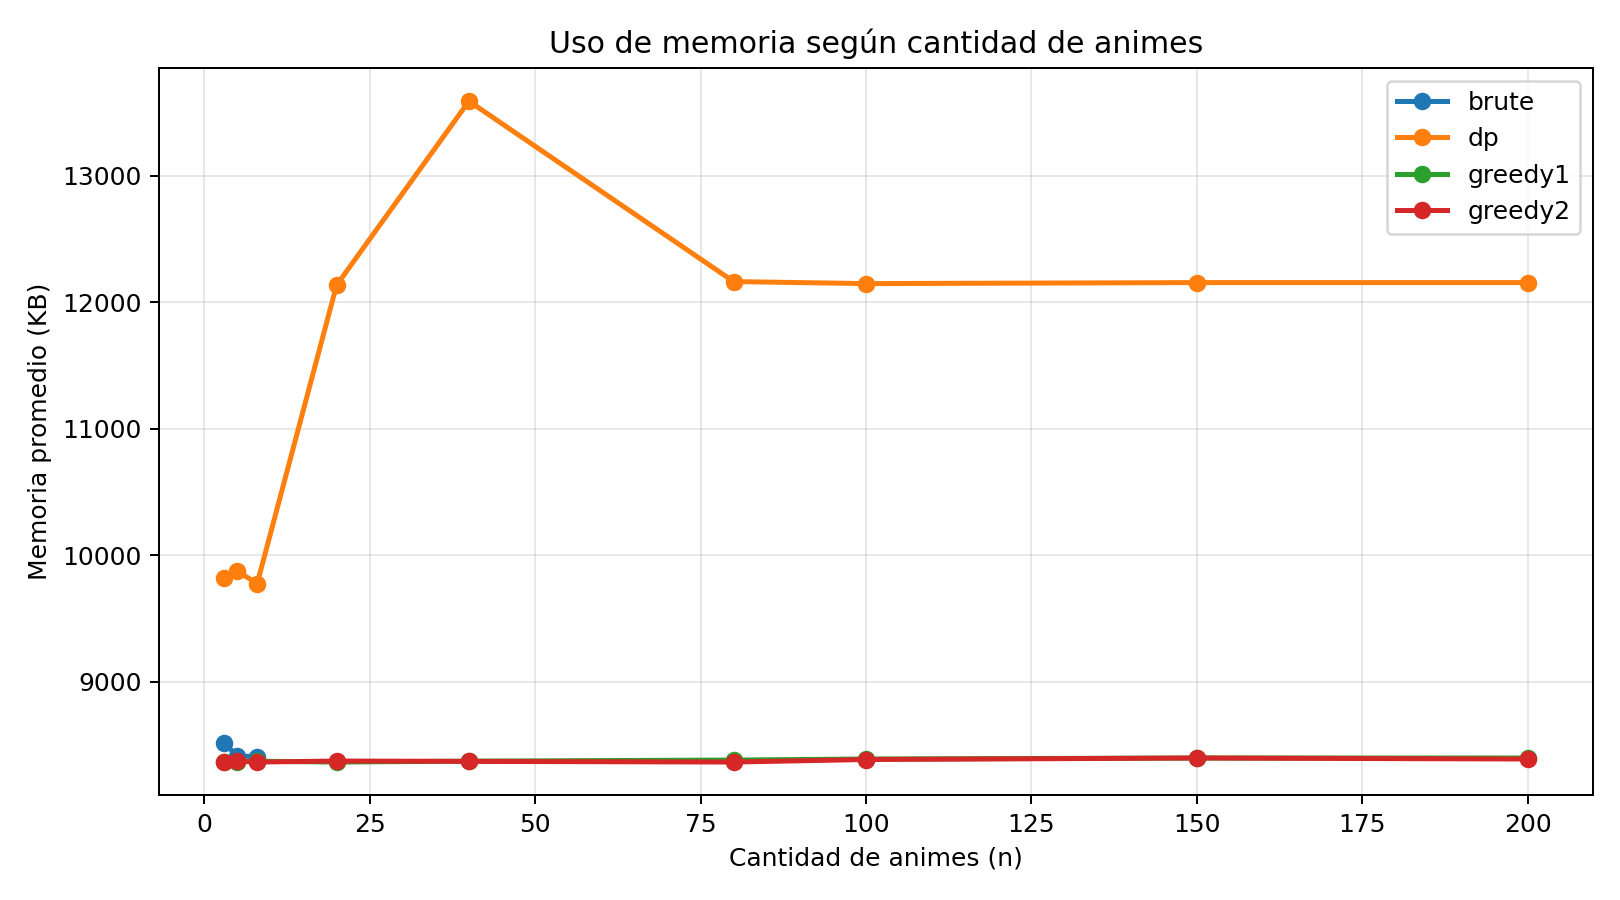
\includegraphics[width=0.92\linewidth]{../code/implementation/data/plots/memoria_vs_n.png}
\caption{Uso de memoria según cantidad de animes.}
\label{fig:memoria_n}
\end{figure}

Las Figuras~\ref{fig:memoria_capitulos}, \ref{fig:memoria_m} y~\ref{fig:memoria_e} muestran que la memoria no varía de forma estrictamente monótona. Esto no necesariamente indica un error: la medición corresponde al \emph{peak working set} reportado por el sistema operativo, por lo que puede verse afectada por el runtime, la reserva interna de memoria y la distribución concreta de cada instancia. En consecuencia, las curvas deben interpretarse como una tendencia general y no como una función exacta del parámetro mostrado en el eje horizontal.

\begin{figure}[ht]
\centering
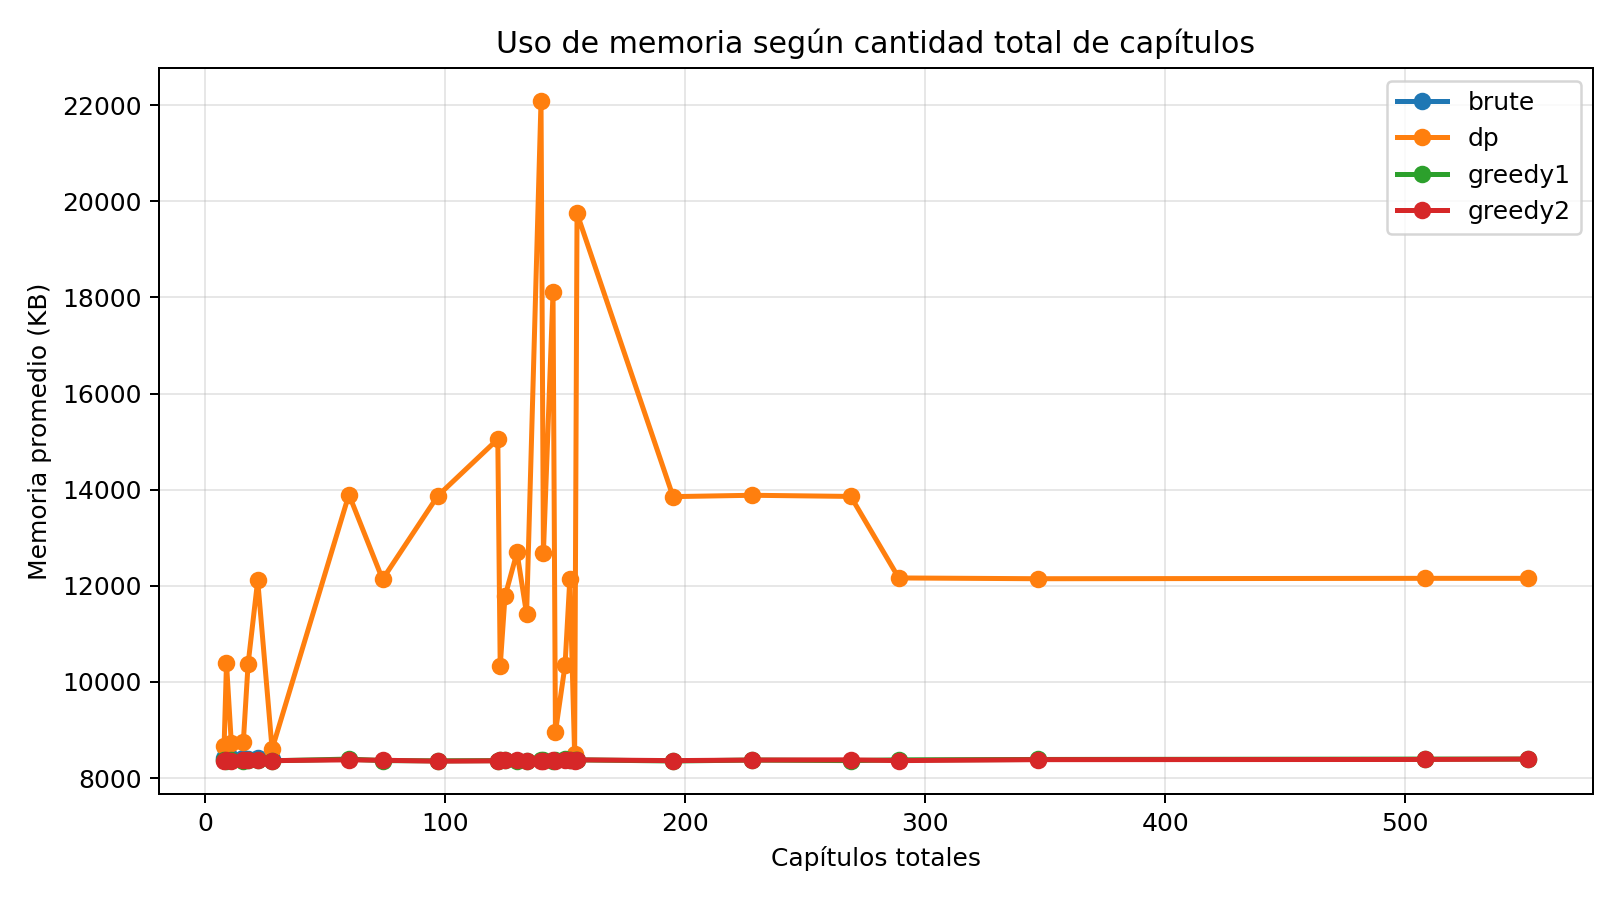
\includegraphics[width=0.92\linewidth]{../code/implementation/data/plots/memoria_vs_capitulos.png}
\caption{Uso de memoria según cantidad total de capítulos.}
\label{fig:memoria_capitulos}
\end{figure}

\begin{figure}[ht]
\centering
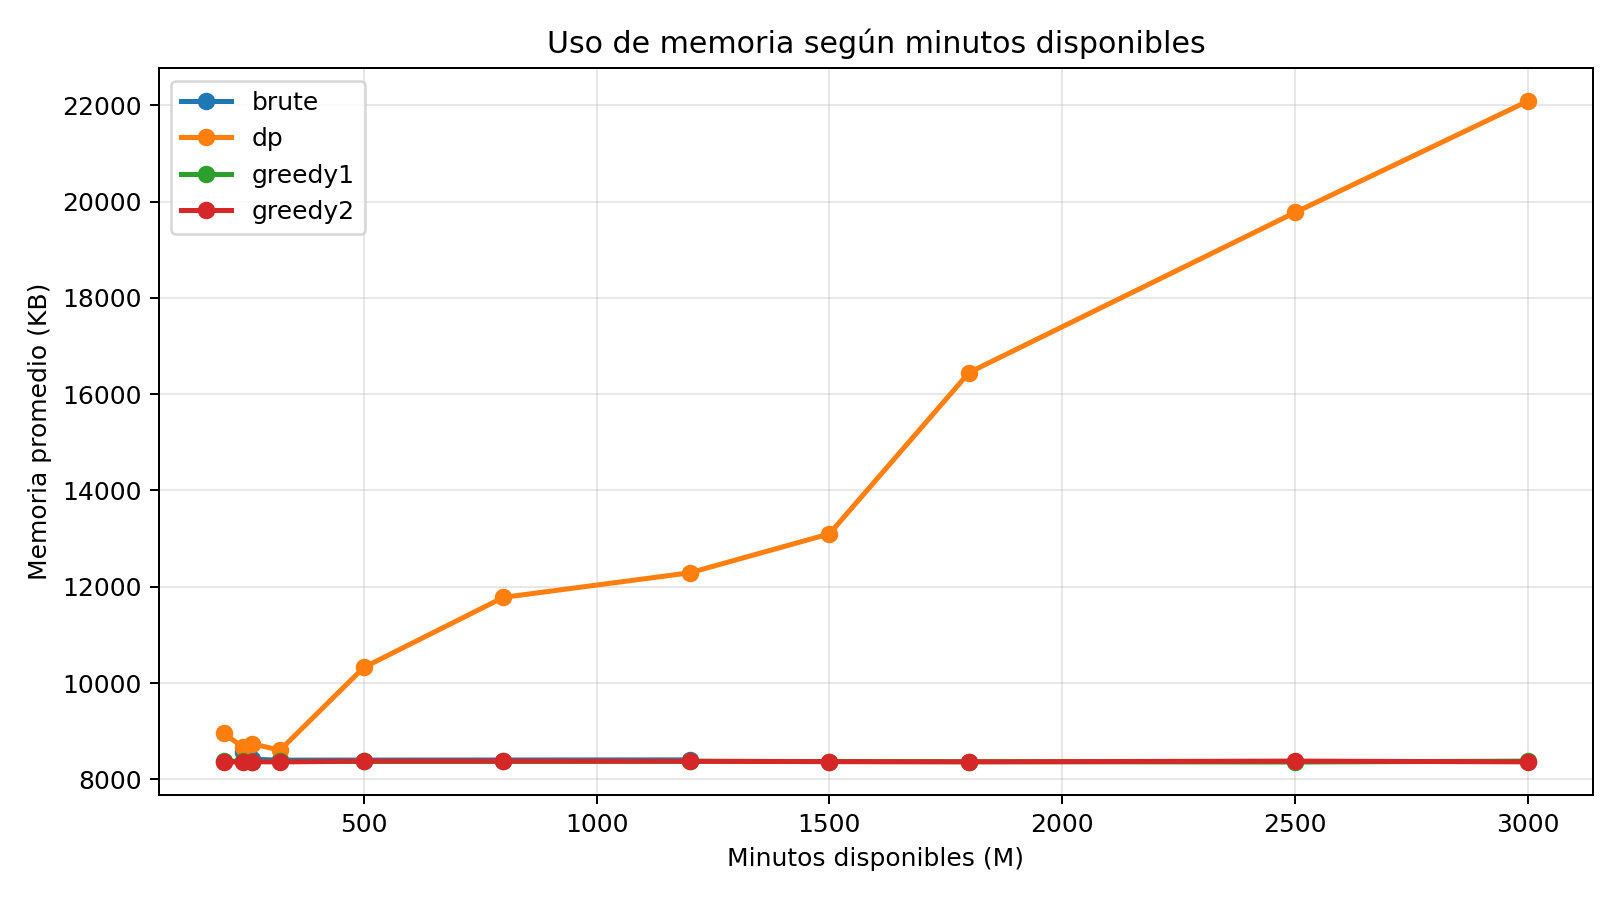
\includegraphics[width=0.92\linewidth]{../code/implementation/data/plots/memoria_vs_M.png}
\caption{Uso de memoria según minutos disponibles.}
\label{fig:memoria_m}
\end{figure}

\begin{figure}[ht]
\centering
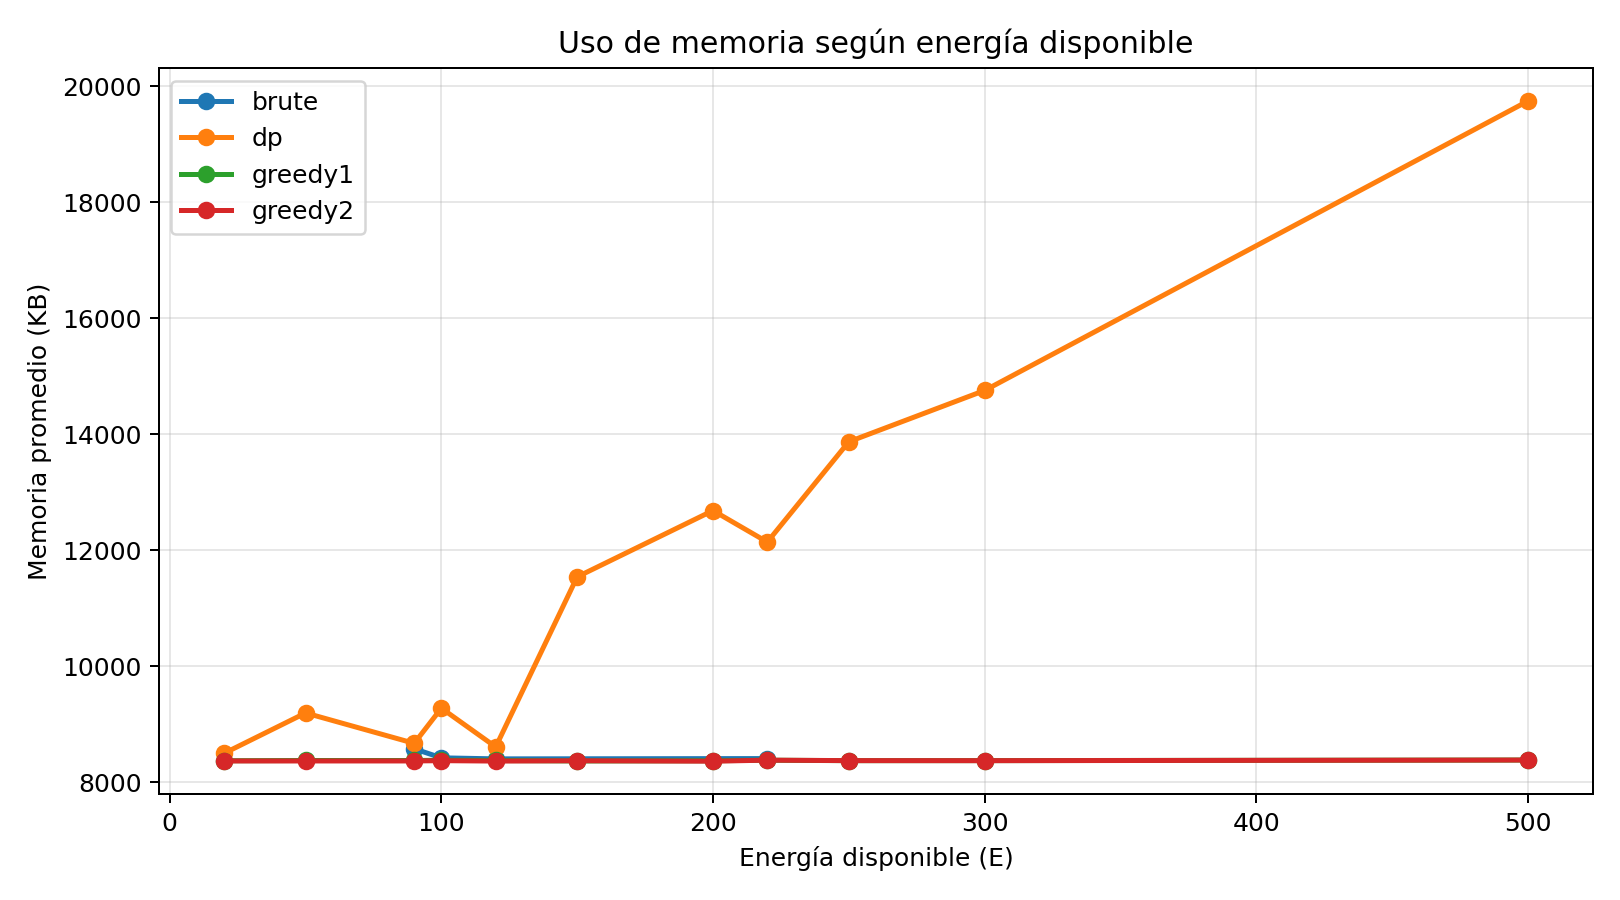
\includegraphics[width=0.92\linewidth]{../code/implementation/data/plots/memoria_vs_E.png}
\caption{Uso de memoria según energía disponible.}
\label{fig:memoria_e}
\end{figure}

\subsection{Comparación de calidad respecto del óptimo}

La Figura~\ref{fig:calidad} compara la solución de los métodos greedy con el óptimo entregado por programación dinámica, usando la razón
[
\text{calidad} = \frac{\text{valor greedy}}{\text{valor óptimo}}.
]
Como la referencia óptima proviene de DP, el valor 1 representa igualdad con la mejor solución encontrada. Se observa que \texttt{greedy2} suele mantenerse más cerca de 1 que \texttt{greedy1}, especialmente en instancias medianas y grandes, mientras que \texttt{greedy1} pierde calidad con mayor rapidez. Esto sugiere que el criterio basado en satisfacción por energía es, en este conjunto de pruebas, una heurística más robusta que el criterio basado en satisfacción por minuto.

\begin{figure}[ht]
\centering
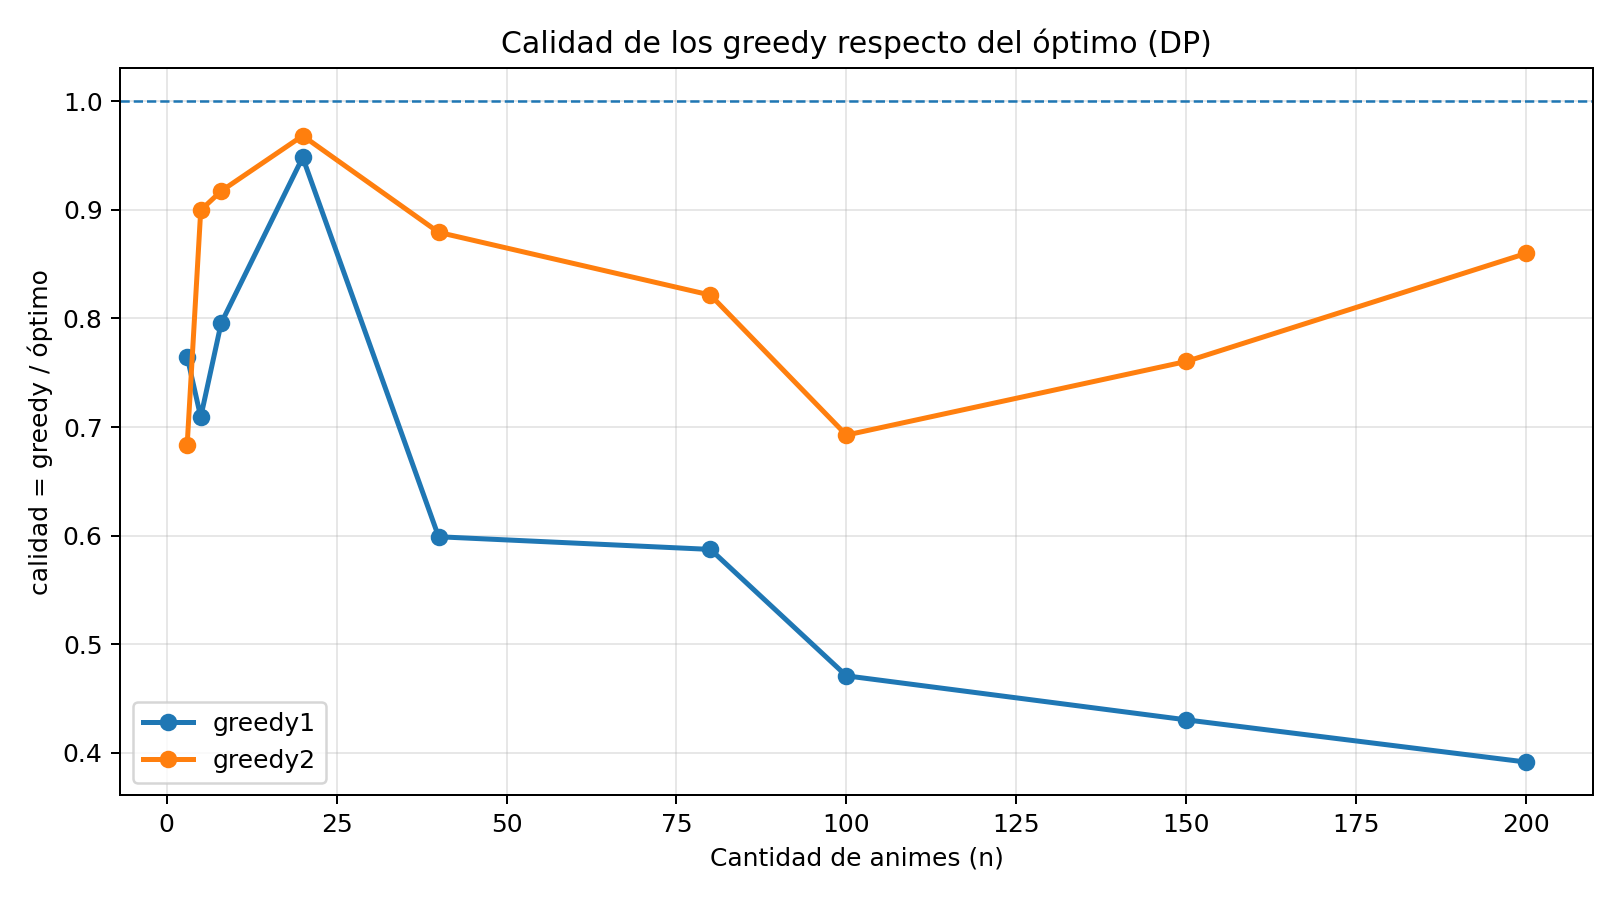
\includegraphics[width=0.92\linewidth]{../code/implementation/data/plots/calidad_greedy_vs_optimo.png}
\caption{Calidad de solución de los greedy respecto del óptimo entregado por programación dinámica.}
\label{fig:calidad}
\end{figure}

\subsection{Comentarios finales sobre las mediciones}

La fuerza bruta solo se ejecutó en instancias pequeñas, porque su costo crece muy rápido y no es razonable exigirle los casos medianos y grandes. En cambio, programación dinámica entrega la referencia exacta para comparar correctitud y calidad, mientras que los métodos greedy permiten estudiar el trade-off entre rapidez y precisión. En conjunto, las mediciones muestran el comportamiento esperado: exactitud a mayor costo para DP, y rapidez con menor calidad para las heurísticas.
